\documentclass[
    ../../Software_Engineering_Summary.tex,
]
{subfiles}

\externaldocument[ext:]{../../Software_Engineering_Summary.tex}
% Set Graphics Path, so pictures load correctly
\graphicspath{{../../}}

\begin{document}
\section{Maintenance \& Evolution}
\subsection{Maintenance}
Software itself doesn't age or degrade. The environment it is deployed in does. Additionally deployed software, however well tested, can have bugs, or might need to change due to changing requirements or new features.

\subsubsection{Triggers for Maintenance}
\begin{defbox}
    [Bug Fixes]
	Most common reason for maintenance. 

    Need to be careful though:
    \begin{itemize}
        \item Extensive testing essential to avoid \defc{regressions}
        \item Accumulate several fixes, decide on an \defc{update schedule}
        \begin{itemize}
            \item Frequent updates annoy users
            \item Deploying new software version can be \defc{expensive}
            \item Providing \defc{change log} is important
        \end{itemize}
        \item Use a \defc{ticket system} to coordinate and prioritize bug fixes
    \end{itemize}
\end{defbox}

\begin{defbox}
    [Changing Requirements]
	Changing requirements \defc{during development} has killed many projects. 

    \defc{Post deployment} though, it is almost inevitable to need to change requirements.
    \begin{itemize}
        \item Changed legal requirements
        \item Changed processes, usage modality
        \item Feedback from users (may indicate insufficient validation)
    \end{itemize}

    \defc{Performance} Requirements:
    \begin{itemize}
        \item Growing user base
        \item Growing amount of data
        \item Usually less of an issue when \defc{cloud-based} architecture is used
    \end{itemize}

    Changed requirement often is actually a new feature
    \begin{itemize}
        \item Is the new functionality required? Is there a business case?
        \item Do previous versions still need to be maintained?
    \end{itemize}
\end{defbox}

\begin{defbox}
    [New Features]
	Features are often requested by clients and users. If these requests should be considered is tricky.

    New features should \defc{add value}, \defc{not merely novelty}.

    Another case might be new customers, who have different requirements.

    This, of course would lead to a new variant of the software, which may be seperate from the current version. But both would need to be deployed and maintained.
\end{defbox}

\begin{defbox}
    [Evolving Hardware]
	\begin{itemize}
    \item \defc{Multiple cores} enable parallel processing
    \item New \defc{hardware architecture}, e.g. x86 $\Rightarrow$ ARM
    \item \defc{Periphery}
    \begin{itemize}
        \item Screens: Resolution, screen size, layout may affect GUI
        \item Storage: Might influence backup requirements
        \item Authentication: Biometrics, 2FA, etc.
        \item New types of sensors: Accelerometer, Magnetometer, etc.
    \end{itemize}
\end{itemize}

How often changes in hardware affect software can be mitigates by picking a suitable architecture or judicious use of design patterns in development.
\end{defbox}

\begin{defbox}
    [Evolving Software Architecture]
	\begin{minipage}
        [c]{0.4\textwidth}
        \centering
        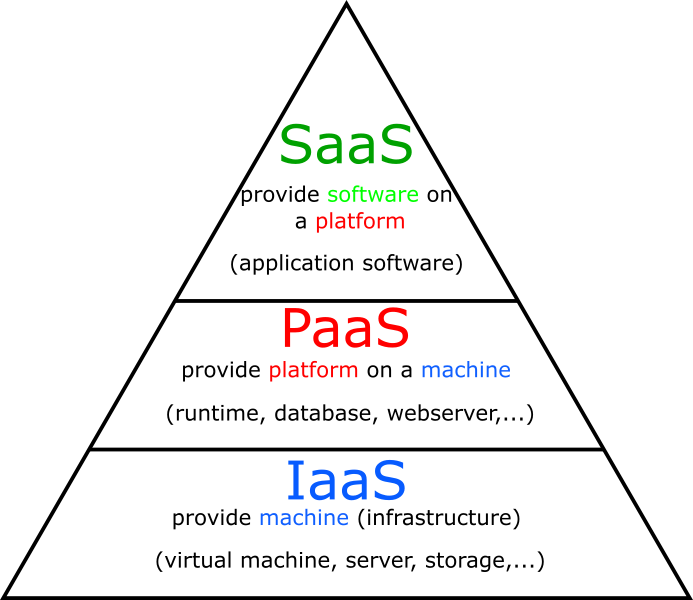
\includegraphics[width = \textwidth]{Pics/12/SoftwareArchitecture.png}
    \end{minipage}
    \begin{minipage}
        [c]{0.6\textwidth}
        \begin{itemize}
            \item Cloud Services: IaaS, PaaS, SaaS:
            \begin{itemize}
                \item[+] \color{codegreen}Cost saving, mobility, scalability\color{black}
                \item[-] \color{codered}Privacy, granularity of interfaces, latency, dependability \color{black}
            \end{itemize}
            \item Virtualization:
            \begin{itemize}
                \item[+] \color{codegreen} Platform independence, enabler of cloud services\color{black}
                \item[-] \color{codered} Performance overhead, not everything is virtualizable, initial cost \color{black}
            \end{itemize}
        \end{itemize}
    \end{minipage}
\end{defbox}

\begin{defbox}
    [Evolving Software Stack]
	\begin{itemize}
    \item \defc{External} software libraries
    \begin{itemize}
        \item Libraries not provided by API of implementation language
    \end{itemize}
    \item Programming language
    \begin{itemize}
        \item Mostly downwards-compatible
        \item Old version not supported indefinitely
    \end{itemize}
    \item \defc{Database} technology
    \begin{itemize}
        \item External $\Rightarrow$ in-memory
        \item Move business logic inside database to gain performance
    \end{itemize}
\end{itemize}
\end{defbox}

\newpage
\subsection{Evolution}
Complex, repeated maintenance actions constitute \defc{software evolution}.

\begin{defbox}
    [Software Evolution]
    The series of changes, new versions, adaptations that occur during software maintenance from inception to initial deployment until final retirement.
\end{defbox}

\subsubsection{Critical Issues in Software Evolution}
\begin{itemize}
    \item \defc{Break} existing functionality. Can be mitigated trough:
    \begin{itemize}
        \item Thorough \defc{regression testing} - Allocate more time for testing than bug fixing
        \item (Possibly) Release \defc{early access} or \defc{beta versions} for experienced users 
    \end{itemize}
    \item Disconnect between specification, documentation, implementation. Mitigation:
    \begin{itemize}
        \item Changed requirements and new features initiate full development cycle
        \item Update requirements specification, use case analysis, etc.
    \end{itemize}
\end{itemize}

\subsubsection{Software Variability}
Excessive changes warrant a new \defc{product variant}:
\begin{itemize}
    \item Changes in user \defc{data format}: Always problematic
    \item Changes in \defc{user interface}: Can invalidate work flow
    \item Loss of compatibility with previous incarnations
    \item[$\Rightarrow$] \defc{Old} and \defc{new} version must both be maintained
\end{itemize}

Need to manage development fork that results in multiple products variants

\subsection{Software Variability Engineering}
\begin{defbox}
    [Software Variability Engineering]
    The necessity to maintain a large number of closely related product variants with differing requirements and features
\end{defbox}

\subsubsection{Challenges in Variability}
\begin{defbox}
    [Product Variability in General]
    \begin{itemize}
        \item Possibly ver large number of variants
        \begin{itemize}
            \item Not all will be realized or even are realizable
        \end{itemize}
        \item Requirements may conflict with each other
    \end{itemize}
\end{defbox}

\begin{defbox}
    [Variability Challenges in Software]
    \begin{itemize}
        \item Keep requirements, documentation, implementation in sync \defc{for each variant} (higher complexity than physical products)
        \item Propagate \defc{bug fixes} to all affected variants (faster frequency)
    \end{itemize}
\end{defbox}

\subsubsection{Software Product Lines}
\begin{defbox}
    [Software Product Lines]
    A collection of software systems that share \defc{common resources} and use a \defc{common means of production}.
\end{defbox}

Typical commonality:
\begin{itemize}
    \item Code basis of \defc{core functionality}
    \item \defc{Architecture}
    \item implementation \defc{programming language(s)}
\end{itemize}

\subsubsection{Terminology of Software Product Line Engineering (SPLE)}
\begin{defbox}
    [Software Feature]
    A distinguishing characteristic of a software item (e.g. performance, portability, functionality)
\end{defbox}

\begin{defbox}
    [Product]
    A set of feature selections and parameter instantiations sufficient to produce executable code from a software product line
\end{defbox}

\begin{defbox}
    [Variant]
    Executable code that implements one product from a software product line
\end{defbox}

\subsubsection{SPLE Schema}
The goal of \defc{Software Product Line Engineering (SLPE)} is to avoid having to maintain each variant seperately.

\begin{defbox}
    [SPLE Principle]
    \begin{enumerate}
        \item Design of the feature space is seperate activity from software design and performed in advance, complementing analysis phase
        \item Same feature should be implemented \defc{not more than once}
        \item It must be possible to \defc{locate} the code that implements a given feature
    \end{enumerate}
\end{defbox}

\begin{figure}
    [H]
    \centering
    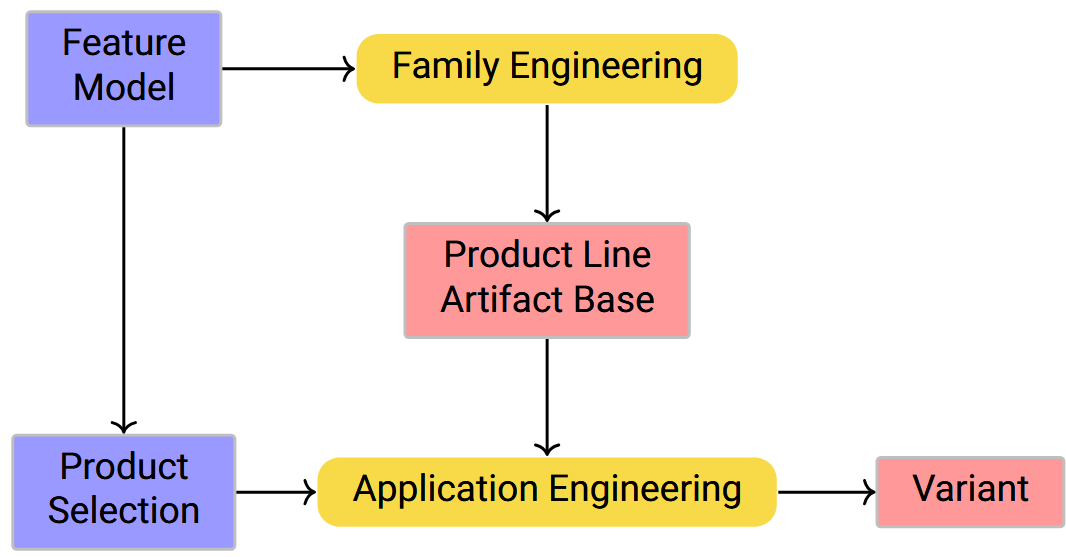
\includegraphics[width = 0.7\textwidth]{Pics/12/SPLESchema.png}
\end{figure}

\subsubsection{Feature Diagrams}
\begin{minipage}
    [c]{0.35\textwidth}
    \centering
    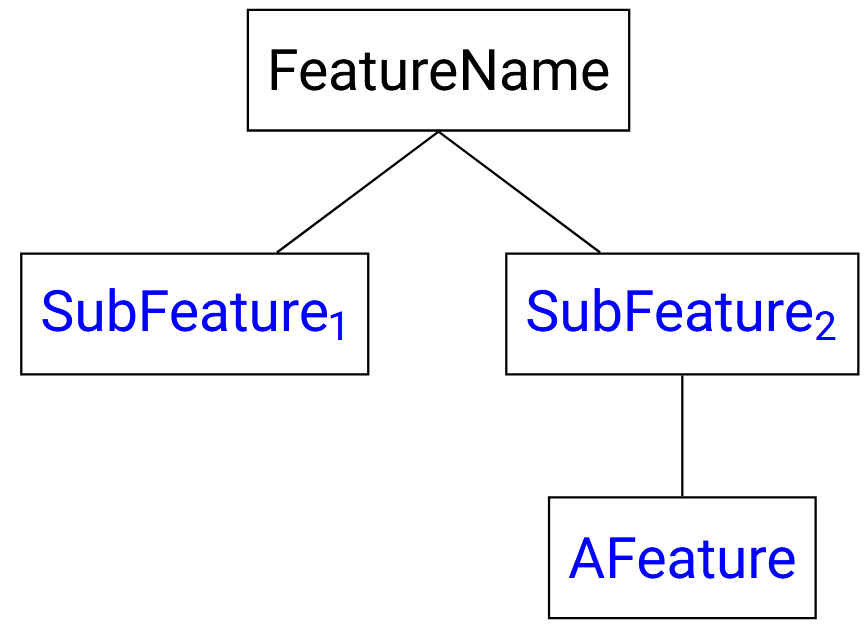
\includegraphics[width = \textwidth]{Pics/12/FeatureDiagramDefault.png}
\end{minipage}
\begin{minipage}
    [c]{0.65\textwidth}
    \begin{itemize}
        \item Top is \defc{root feature}
        \item \defc{Sub feature} only present if parent present
        \item \defc{One or more} sub features selectable
        \item ''AND'' $\land$ connection is the default.
    \end{itemize}

    \vspace{10pt}
    This diagram can also be represented as a \defc{Boolean Integer Formula}:
    
    \begin{defbox}
        [Boolean Integer Formula]
        FeatureName $\land$ (FeatureName $\leftrightarrow$ SubFeature$_1$) $\land$\\ (FeatureName $\leftrightarrow$ SubFeature$_2$) $\land$ (SubFeature$_2$ $\leftrightarrow$ AFeature)
    \end{defbox}
\end{minipage}

\begin{minipage}
    [c]{0.35\textwidth}
    \centering
    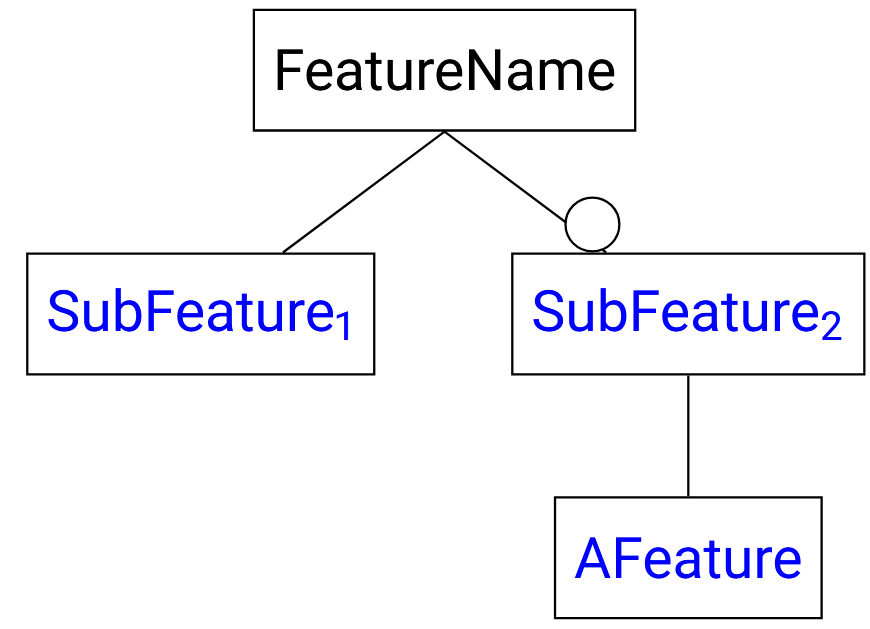
\includegraphics[width = \textwidth]{Pics/12/FeatureDiagramOptional.png}
\end{minipage}
\begin{minipage}
    [c]{0.65\textwidth}
    $\circ$ denotes an \defc{optional feature}

    \begin{defbox}
        [Boolean Integer Formula]
        FeatureName $\land$ (FeatureName $\leftrightarrow$ SubFeature$_1$) $\land$\\ \defc{(FeatureName $\rightarrow$ SubFeature$_2$)} $\land$ (SubFeature$_2$ $\leftrightarrow$ AFeature)
    \end{defbox}
\end{minipage}

\begin{minipage}
    [c]{0.35\textwidth}
    \centering
    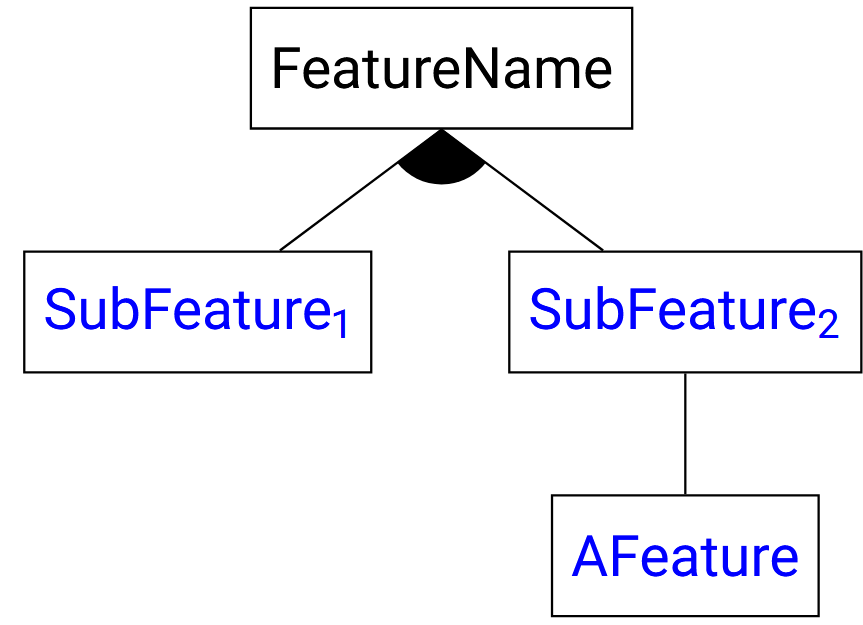
\includegraphics[width = \textwidth]{Pics/12/FeatureDiagramOR.png}
\end{minipage}
\begin{minipage}
    [c]{0.65\textwidth}
    \tikz{\filldraw[fill=black, rotate=180] (0,0) arc[start angle=0, end angle=180, radius=1ex] -- cycle;} denotes an \defc{OR $\lor$ connection}

    \begin{defbox}
        [Boolean Integer Formula]
        FeatureName $\land$ (FeatureName $\leftrightarrow$ (SubFeature$_1$ $\lor$ SubFeature$_2$))\\ $\land$ (SubFeature$_2$ $\leftrightarrow$ AFeature)
    \end{defbox}
\end{minipage}

\begin{minipage}
    [c]{0.35\textwidth}
    \centering
    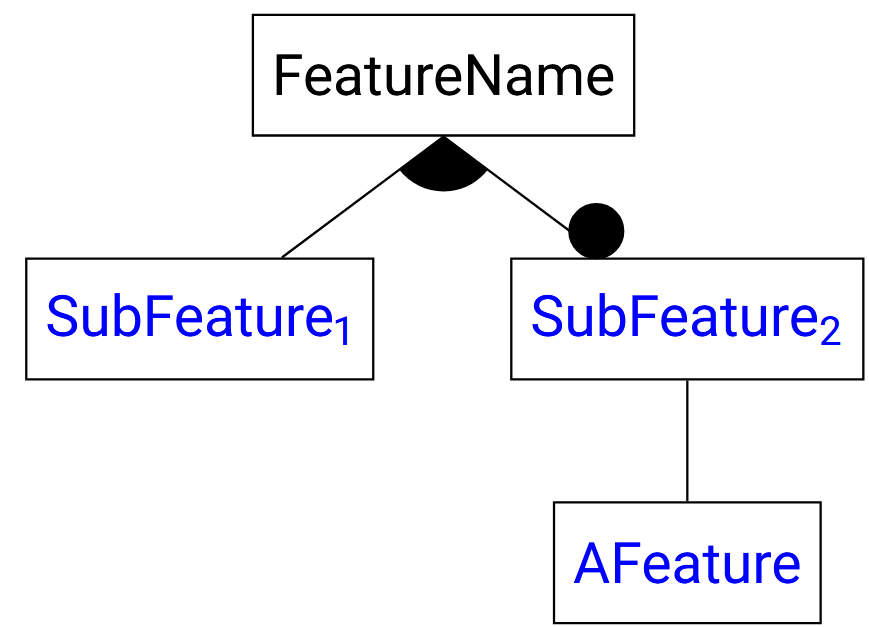
\includegraphics[width = \textwidth]{Pics/12/FeatureDiagramMandatory.png}
\end{minipage}
\begin{minipage}
    [c]{0.65\textwidth}
    $\bullet$ denotes a \defc{mandatory feature}

    \begin{defbox}
        [Boolean Integer Formula]
        FeatureName $\land$ (FeatureName $\leftrightarrow$ (SubFeature$_1$ $\lor$ SubFeature$_2$))\\ $\land$ \defc{(FeatureName $\leftrightarrow$ SubFeature$_2$)} $\land$ (SubFeature$_2$ $\leftrightarrow$ AFeature)
    \end{defbox}
\end{minipage}

\begin{minipage}
    [c]{0.35\textwidth}
    \centering
    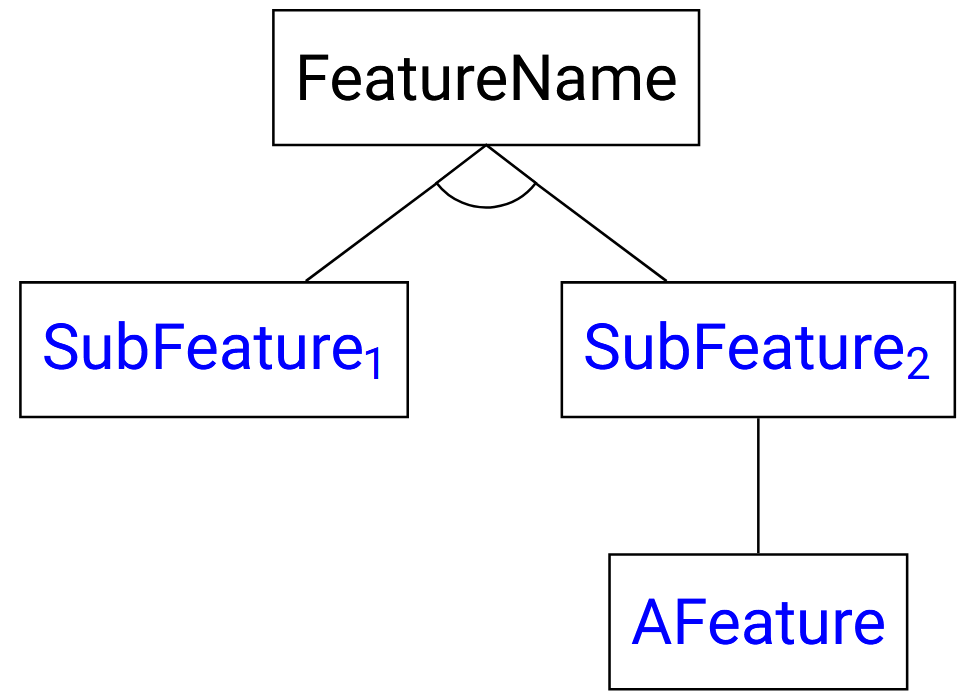
\includegraphics[width = \textwidth]{Pics/12/FeatureDiagramAlternative.png}
\end{minipage}
\begin{minipage}
    [c]{0.65\textwidth}
    \tikz{\filldraw[fill=none, rotate=180] (0,0) arc[start angle=0, end angle=180, radius=1ex] -- cycle;} denotes an \defc{alternative feature} (exactly one)

    \begin{defbox}
        [Boolean Integer Formula]
        FeatureName $\land$\\ \defc{(SubFeature$_1$ \leftrightarrow (FeatureName $\land$ $\neg$Subfeature$_2$))} $\land$\\
        \defc{(SubFeature$_2$ \leftrightarrow (FeatureName $\land$ $\neg$Subfeature$_1$))} $\land$\\ (SubFeature$_2$ $\leftrightarrow$ AFeature)
    \end{defbox}
\end{minipage}

\begin{minipage}
    [c]{0.35\textwidth}
    \centering
    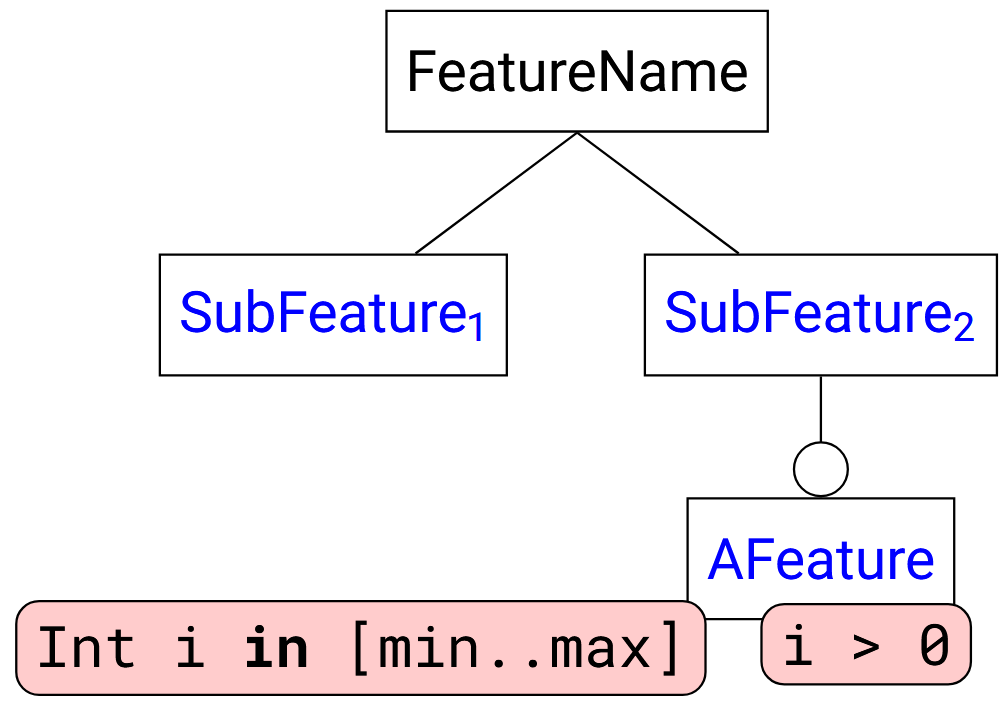
\includegraphics[width = \textwidth]{Pics/12/FeatureDiagramParameter.png}
\end{minipage}
\begin{minipage}
    [c]{0.65\textwidth}
    Denotes a \defc{parameter} with type. Can be further specified with
    \begin{itemize}
        \item Range
        \item (Exact) Constraint
    \end{itemize}
    \begin{defbox}
        [Boolean Integer Formula]
        \dots $\land$ (AFeature $\rightarrow$ ($i \geq \min \land  i \leq \max \land  i > 0$))
    \end{defbox}
\end{minipage}

\begin{minipage}
    [c]{0.35\textwidth}
    \centering
    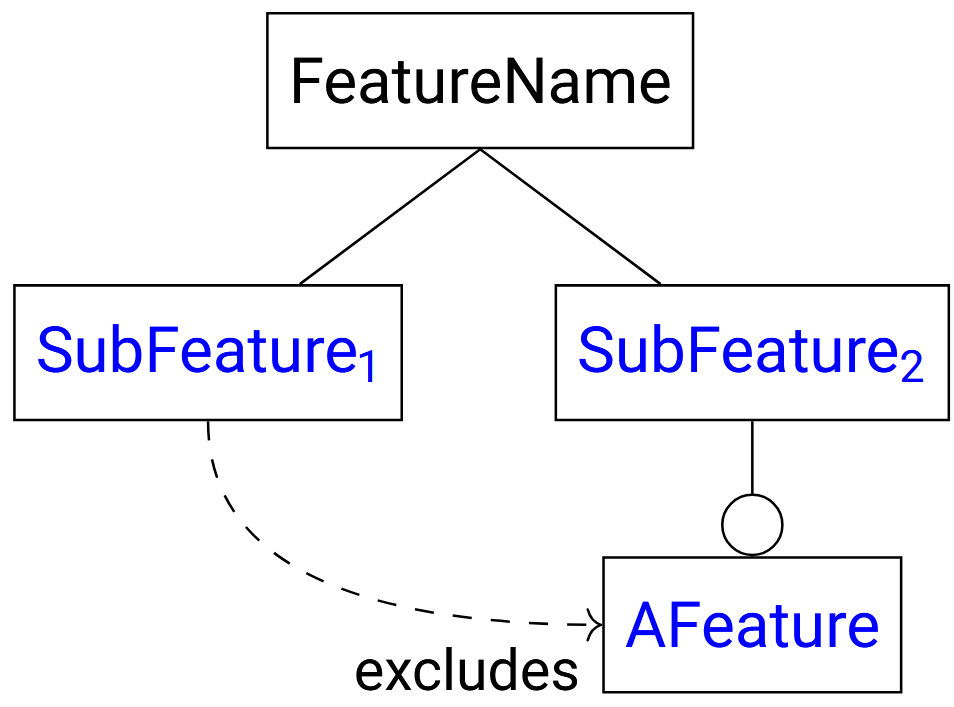
\includegraphics[width = \textwidth]{Pics/12/FeatureDiagramExcludes.png}
\end{minipage}
\begin{minipage}
    [c]{0.65\textwidth}
    This denotes that a feature \defc{excludes} another feature.
    \begin{defbox}
        [Boolean Integer Formula]
        \dots $\land$ (SubFeature$_1$ $\rightarrow$ $\neg$AFeature)
    \end{defbox}
\end{minipage}

\begin{minipage}
    [c]{0.35\textwidth}
    \centering
    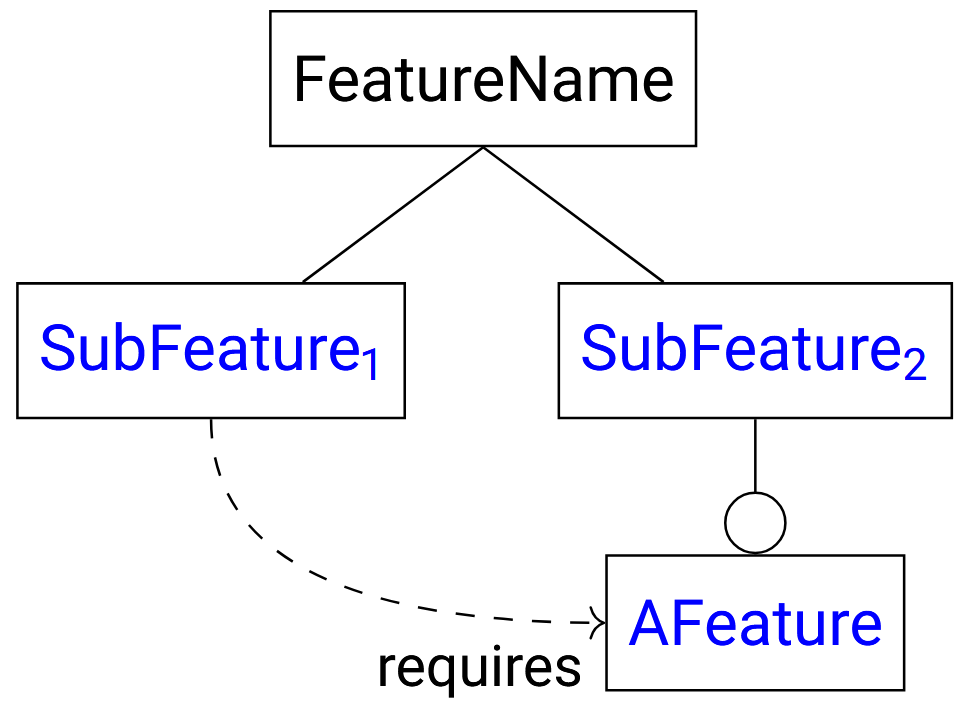
\includegraphics[width = \textwidth]{Pics/12/FeatureDiagramRequires.png}
\end{minipage}
\begin{minipage}
    [c]{0.65\textwidth}
    This denotes that a feature \defc{requires} another feature.
    \begin{defbox}
        [Boolean Integer Formula]
        \dots $\land$ (SubFeature$_1$ $\rightarrow$ AFeature)
    \end{defbox}
\end{minipage}

\subsubsection{Implementing SPLE at Code Level}
Many approaches:
\begin{itemize}
    \item \defc{Conditional activation} of code segment corresponding to feature implementation at compile time
    \item \defc{Aspect-oriented} programming
    \item \defc{Feature-oriented} programming
    \item \defc{Delta-oriented} programming
    \item \defc{Variability modules}
\end{itemize}
All, except conditional activation, require programming language extensions

Usually \defc{conditional activation} is used - despite the challenges.

\subsubsection{Challenges in SPLE}
\begin{itemize}
    \item Code with many pragmas / macros is hard to understand
    \item \defc{Feature interaction} may occur, but is hard to detect
    \begin{itemize}
        \item Incompatible features
        \item Ambigous behaviour depending on sequence of activation
    \end{itemize}
    \item Not easy to avoid \defc{code duplication}: Same code used in many features
    \begin{itemize}
        \item Can be mitigated by \defc{code reuse mechanisms}, such as \defc{traits}
    \end{itemize}
    \item Analysis, \defc{testing}, \defc{type checking} difficult at product line level
    \begin{itemize}
        \item Faults detected only when variant is \defc{created}, not during design
    \end{itemize}
\end{itemize}

\subsubsection{Product Line Artifact Base}
When available: Use Conditional Compilation / Macros

\begin{defbox}
    [Conditional Compilation / Macros]
    Use primitives like \texttt{\#ifdef} and \texttt{\#elif} to mark code regions that are only comiled if a condition (a feature is selected) is satisfied
\end{defbox}

Design code base with (known) extensiblity in mind

\begin{defbox}
    [Extensible Code Base]
    \begin{itemize}
        \item Identify suitable OO \defc{abstractions} (interfaces, abstract classes)
        \item Implement variants as new implementations of interfaces
        \item Design patterns make software structure and behaviour extensible
    \end{itemize}
\end{defbox}

Build automation / deployment tools e.g. KConfig, Gradle, configure\dots

\begin{defbox}
    [Build Automation Tools]
    \begin{enumerate}
        \item Organize variant code in seperate files, directories, modules
        \item Configure automated build tool to
        \begin{itemize}
            \item define \defc{products} as build \defc{targets}
            \item model \defc{features} in the tools \defc{domain specific language (DSL)}
            \item \defc{merge} common code base and artifacts using \defc{build tool actions}
        \end{itemize}
    \end{enumerate}
\end{defbox}

\begin{codebox}
    [Example: Linux Kernel - Human Interface Driver]
    \begin{lstlisting}[language=C]
#ifdef CONFIG_HID_APPLE_MODULE
        HID_COMPAT_CALL_DRIVER(apple);
#endif
...
    \end{lstlisting}
    enables the Apple HID driver if feature \texttt{HID\_APPLE} is selected

    Features and their relations are defined in kernel configuration file:
    \begin{lstlisting}[language=C]
config HID_APPLE tristate "Apple"
default m # comiled by default
depends on (USB_HID || BT_HIDP) help
    \end{lstlisting}

    Feature \texttt{HID\_APPLE} \defc{requires} feature \texttt{USB\_HID} \defc{or} feature \texttt{BT\_HIDP} to be enabled
\end{codebox}
\end{document}